\documentclass{article}
\usepackage{neurips_2025}
\usepackage[utf8]{inputenc}
\usepackage[T1]{fontenc}
\usepackage{hyperref}
\usepackage{url}
\usepackage{booktabs}
\usepackage{amsmath,amsfonts}
\usepackage{graphicx}
\usepackage{microtype}
\usepackage{xcolor}
\usepackage{multirow}
\usepackage{array}

\title{The Power of Prior Revisited:\\
Training-Free Open-Vocabulary Segmentation with LLaVA}

\author{Anonymous Authors}

\newcommand{\method}{FSeg-LLaVA}
\newcommand{\miou}{mIoU}

\begin{document}

\maketitle

\begin{abstract}
Training-free open-vocabulary segmentation asks a frozen vision-language model (VLM) to provide
semantic and spatial evidence that can be converted into pixel masks without segmentation-specific
fine-tuning. We independently reimplement and evaluate the \method{} framework, which extracts
class-conditioned spatial priors from LLaVA and uses them to prompt the frozen Segment Anything
Model (SAM). On all 1,449 PASCAL VOC 2012 validation images, our Hugging Face implementation
achieves 65.85 VOC21 \miou{}, close to the paper's 68.0 and to 66.01 from the released
implementation. The method transfers across LLaVA versions: LLaVA-1.6 Vicuna and Mistral obtain
65.02 and 66.29 \miou{}, respectively. On 5,000 COCO-Object images, the same pipeline obtains
39.99 \miou{}. Oracle class recognition raises performance to 69.46, 70.00, and 50.41 on the
two VOC model variants and COCO, respectively. These gaps show that class-presence recognition,
rather than mask refinement alone, is the dominant bottleneck. Layer-wise analysis further shows
that middle-layer maps are compact and precise seeds for SAM, whereas deeper maps have better
standalone coverage but less useful prompts. Our contribution is a controlled reproduction and
cross-model, cross-dataset analysis that identifies where the training-free prior succeeds and
where it fails.
\end{abstract}

\section{Introduction}
\label{sec:introduction}
Open-vocabulary semantic segmentation requires a system to assign pixels to classes specified at
inference time. Conventional segmentation systems achieve strong accuracy by training on
pixel-level annotations, but this makes their class vocabulary and deployment cost restrictive.
Recent vision-language models (VLMs) contain broad semantic knowledge and image-text alignment,
while promptable segmenters such as SAM provide high-quality masks from sparse spatial prompts.
The \method{} framework combines these capabilities without training a segmentation head:
LLaVA answers whether a candidate class is present and its internal representations provide a
coarse spatial prior; SAM turns that prior into pixel masks.

This work studies whether the proposed mechanism is reproducible and whether its spatial prior
generalizes beyond the exact model and dataset used in the original paper. We ask:
\begin{enumerate}
    \item Can the published result be reproduced in an independent Transformers implementation?
    \item Which implementation details and LLaVA layers determine the quality of SAM prompts?
    \item Does the method transfer across LLaVA variants and from VOC to COCO-Object?
    \item Is final performance limited primarily by recognition or by mask generation?
\end{enumerate}

Our study makes four empirical contributions. First, we provide a controlled reproduction on the
complete VOC validation split and compare against the released implementation. Second, we separate
recognition, localization, and SAM refinement through coarse-map and oracle-class experiments.
Third, we perform a layer-wise study that distinguishes seed precision from standalone map
coverage. Fourth, we evaluate multiple LLaVA variants and a larger, more diverse COCO-Object
benchmark. We deliberately present this as a reproduction-plus-analysis study, not as a claim to
have invented the original segmentation algorithm.

\section{Literature Review}
\label{sec:literature}
\paragraph{Vision-language models.}
CLIP-style contrastive pretraining aligns image and text representations, while instruction-tuned
models such as LLaVA connect a vision encoder to a large language model for visual question
answering. These models are trained for semantic understanding rather than pixel-level prediction,
but their image-token representations can retain spatial information.

\paragraph{Open-vocabulary segmentation.}
Open-vocabulary and referring segmentation methods typically transfer image-text alignment to
dense prediction, often using additional training, region proposals, or specialized decoders.
Training-free approaches instead exploit frozen representations and prompting, making them useful
for studying the latent spatial capabilities of general-purpose VLMs.

\paragraph{Promptable segmentation.}
SAM is a general-purpose promptable segmenter trained on large-scale mask data. It does not decide
which object class is present; it refines points, boxes, and masks into object boundaries. The
\method{} pipeline therefore separates semantic recognition and localization from boundary
generation.

\paragraph{Position of this work.}
The original \method{} paper demonstrates the core pipeline. We extend its evaluation with an
independent implementation, explicit paper-versus-code ablations, oracle recognition controls,
layer diagnostics, cross-version model comparisons, and COCO-Object transfer. This makes the
failure modes and generalization limits measurable rather than attributing all errors to the
segmentation stage.

\section{Problem Statement}
\label{sec:problem}
Given an image $I$ and a candidate vocabulary $\mathcal{C}$, the goal is to predict an indexed
mask $\hat{Y}: I \rightarrow \{0,\ldots,|\mathcal{C}|\}$ without training on segmentation labels
for the target vocabulary. The system may use frozen pretrained models, but the inference
procedure must determine which classes are present and where their pixels occur.

We evaluate with mean intersection-over-union:
\[
\miou{} = \frac{1}{|\mathcal{C}|+1}\sum_{c=0}^{|\mathcal{C}|}
\frac{|\hat{Y}=c \cap Y=c|}{|\hat{Y}=c \cup Y=c|},
\]
where class $0$ is background and void pixels are ignored. All primary VOC numbers use VOC21
scoring (20 foreground classes plus background), with intersections and unions accumulated over
the complete split.

\section{Proposed Method}
\label{sec:method}
\subsection{Question--answer pipeline}
For each candidate class $c$, LLaVA receives a fixed image question asking whether $c$ is
present. Positive answers are retained and provide the class token and a short description.
Negative answers are discarded. This stage supplies a semantic gate, but it can introduce false
positives and false negatives before any mask is generated.

\subsection{Text--visual response}
Let $h_c^l$ be the hidden state of the class-name token at language-model layer $l$, and let
$h_{i}^{l}$ be the hidden state of image token $i$. We compute class-conditioned spatial scores
from cosine similarities:
\[
D_c(i)=\frac{1}{|L|}\sum_{l\in L}
\frac{h_c^l\cdot h_i^l}{\|h_c^l\|\|h_i^l\|}.
\]
The scores are reshaped to the vision-token grid and thresholded. We additionally use
description-to-image attention to retain spatially coherent evidence. Our default follows the
released implementation where the attention map is combined with the thresholded map by union,
rather than the product described in the paper text.

\subsection{Visual prompting and SAM}
CLIP patch features are used to form class and background prototypes. The resulting coarse mask
provides positive points, a box, and negative points associated with other classes. SAM ViT-H
refines these prompts for three rounds. Candidate masks are selected using overlap with the
class-conditioned prior and then merged using an explicit background policy.

\subsection{Independent implementation}
Our implementation uses Hugging Face Transformers for LLaVA access, explicit token indexing,
cached per-image traces, and a separate evaluation module. Hyperparameters are selected on a
200-image subset of VOC train and frozen before full validation. Oracle experiments replace only
the predicted present-class set with the ground-truth set and are reported as diagnosis, never as
the primary result.

\section{Experiments and Results}
\label{sec:experiments}
\subsection{Experimental setup}
The primary VOC experiments use LLaVA-1.5-7B with SAM ViT-H and all 1,449 VOC2012 validation
images. We also evaluate LLaVA-1.6 Vicuna and Mistral on the same split. The COCO-Object run
contains 5,000 validation images and uses the same training-free pipeline. Experiments run on a
single NVIDIA A30 GPU. No segmentation-specific fine-tuning is performed.

\subsection{Reproduction and model comparison}
\begin{table}[t]
\centering
\caption{VOC21 validation results. ``Coarse'' evaluates the LLaVA spatial prior without SAM.
Oracle recognition supplies the correct present-class set only for diagnosis.}
\label{tab:voc}
\begin{tabular}{lccc}
\toprule
System & Coarse & Standard & Oracle recognition\\
\midrule
Paper-reported LLaVA-1.5 & -- & 68.00 & --\\
Our LLaVA-1.5 reproduction & 18.72 & 65.85 & 72.16\\
Released implementation & -- & 66.01 & --\\
LLaVA-1.6 Vicuna & 16.45 & 65.02 & 69.46\\
LLaVA-1.6 Mistral & 19.90 & 66.29 & 70.00\\
\bottomrule
\end{tabular}
\end{table}

Table~\ref{tab:voc} shows that the independent reproduction is within 2.15 points of the paper
and within 0.16 points of the released implementation. The two LLaVA-1.6 models remain close to
the LLaVA-1.5 reproduction, indicating that the approach is not restricted to one checkpoint.
Mistral is the strongest tested standard model at 66.29 \miou{}.

\subsection{COCO-Object transfer}
\begin{table}[t]
\centering
\caption{COCO-Object validation results on 5,000 images.}
\label{tab:coco}
\begin{tabular}{lc}
\toprule
Configuration & \miou{}\\
\midrule
LLaVA coarse maps only & 18.40\\
Full LLaVA + SAM pipeline & 39.99\\
Oracle recognition + SAM & 50.41\\
\bottomrule
\end{tabular}
\end{table}

The full pipeline transfers to COCO with 39.99 \miou{} despite the larger vocabulary, smaller
objects, and more crowded scenes. SAM improves the coarse prior by 21.59 points. Correct class
recognition would add another 10.42 points, demonstrating that recognition quality becomes even
more important as the vocabulary and visual diversity increase.

\subsection{Ablations and implementation checks}
\begin{table}[t]
\centering
\caption{Selected VOC2012 ablations from the independent LLaVA-1.5 reproduction.}
\label{tab:ablation}
\begin{tabular}{lc}
\toprule
Configuration & VOC21 \miou{}\\
\midrule
Full reproduction & 65.85\\
No prototype step & 65.78\\
No attention mask & 65.49\\
Paper-text map product & 61.62\\
SAM points only & 57.70\\
SAM box only & 54.12\\
Class token shifted one position & 48.57\\
Coarse LLaVA maps only & 18.72\\
\bottomrule
\end{tabular}
\end{table}

The ablations reproduce the qualitative trends in the original work. The union used by the
released code is substantially better than the product written in the paper text. Reading the
class token at the wrong position costs 17.28 points, showing that the spatial prior is sensitive
to exact token alignment. SAM is essential: the coarse map is not a competitive final mask, but
it is a useful prompt for a general-purpose segmenter.

\subsection{Layer-wise analysis}
The layer study separates two properties that are conflated by a single final score. Layers 7--13
produce compact, precise seeds and are effective for SAM prompting. Deeper layers, especially
around 17--22, produce maps with greater standalone coverage but oversized or less selective
prompts. Thus, the layer with the best dense map is not necessarily the layer that gives the best
downstream segmentation. This supports the interpretation that LLaVA's useful spatial prior is
distributed and changes from precise localization to broad semantic coverage across depth.

\subsection{Failure analysis}
On VOC, the largest errors are person close-ups and recognition mistakes for chair, sofa, dining
table, and bottle. In close-ups, LLaVA may localize only a face or skin region, causing SAM to
refine an incomplete prior. The oracle experiments show that correcting recognition alone yields
4.43 points for LLaVA-1.6 Vicuna, 3.71 points for Mistral, and 10.42 points on COCO. This is
evidence that future work should improve the semantic gate and class-conditioned prior, rather
than treating all residual error as a SAM boundary problem.

\begin{figure}[t]
\centering
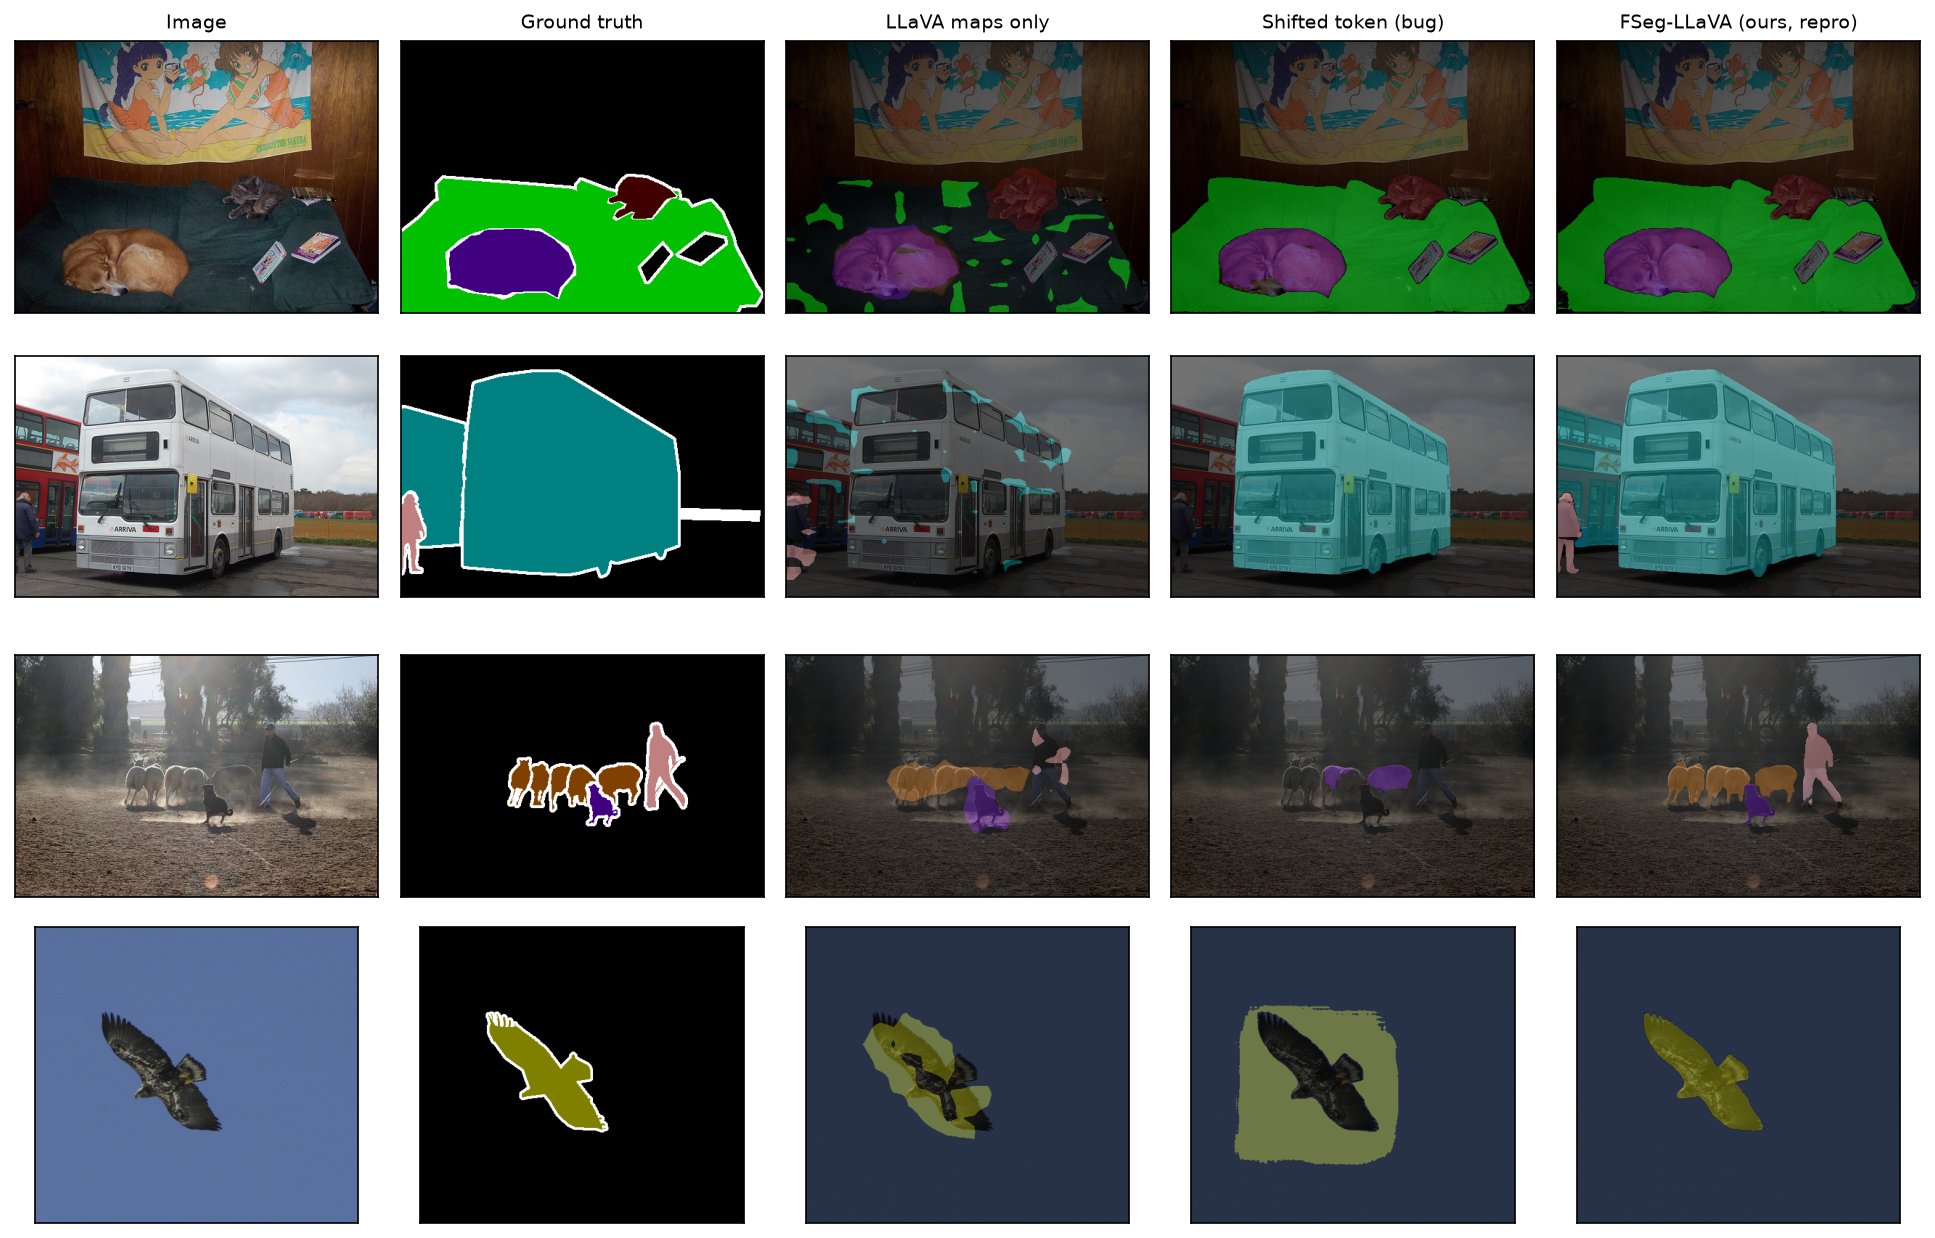
\includegraphics[width=.47\linewidth]{../reports/figures/qualitative_success.png}
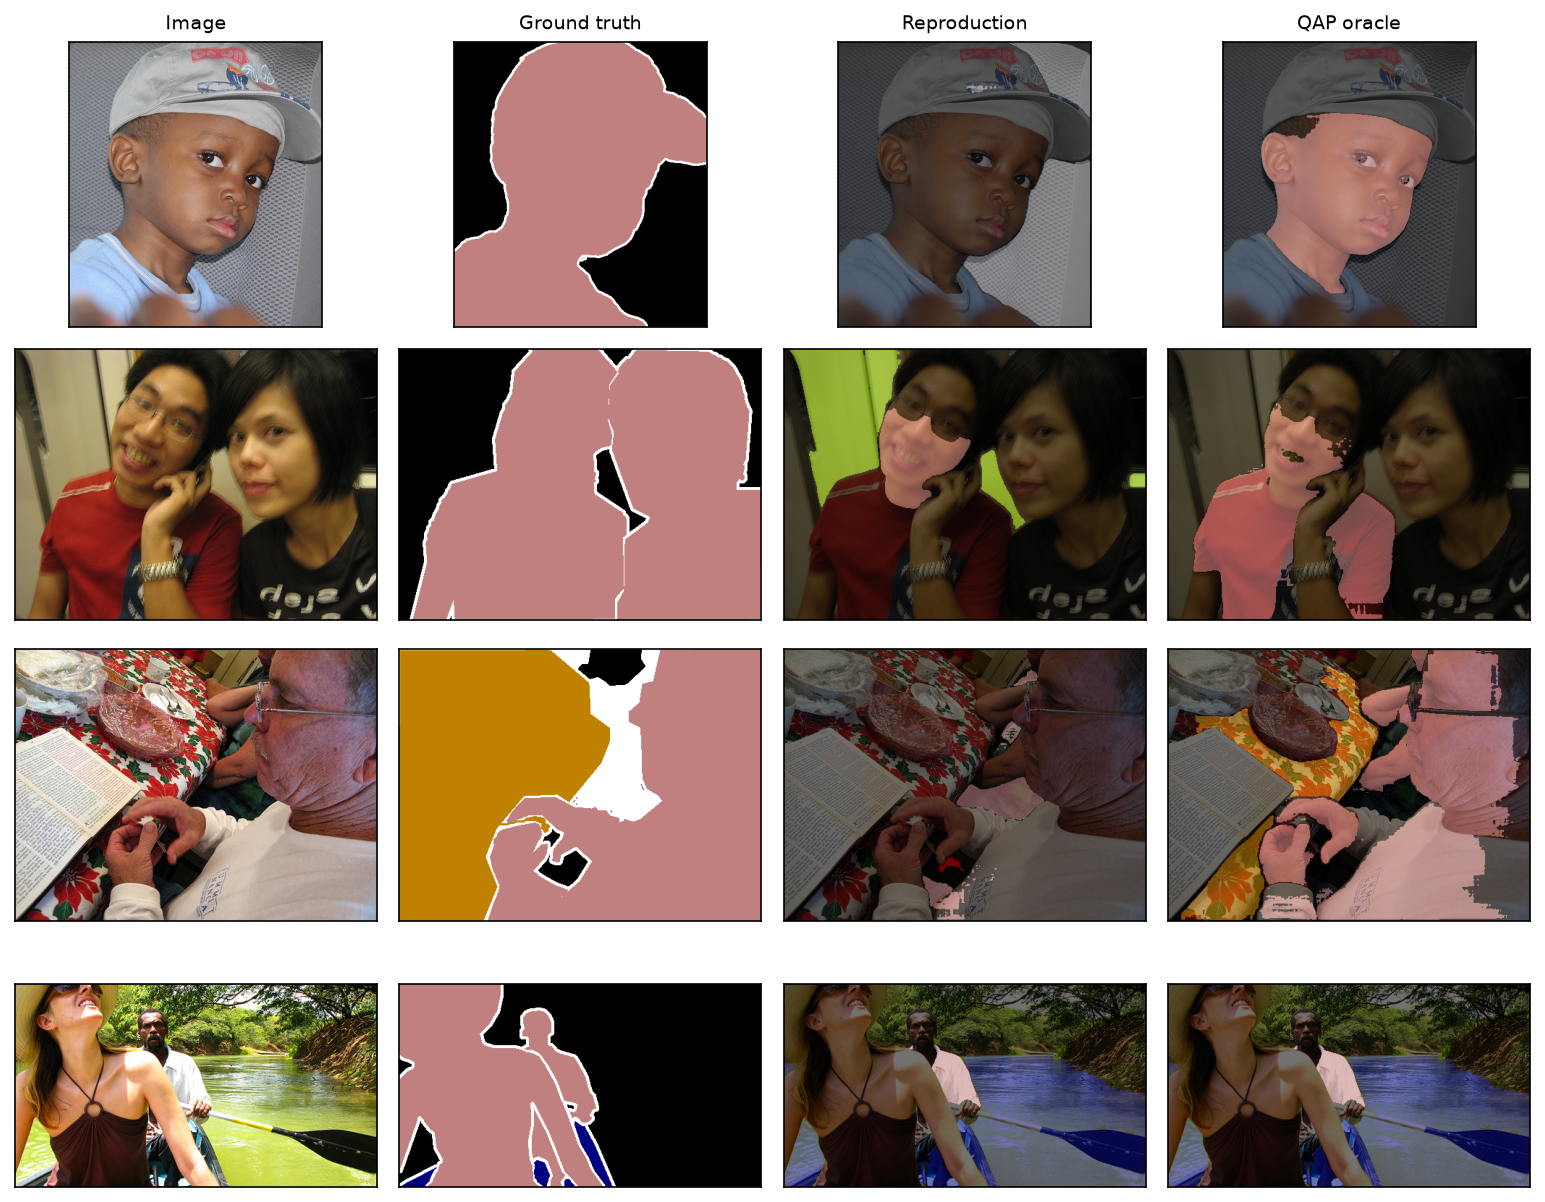
\includegraphics[width=.47\linewidth]{../reports/figures/qualitative_failures.png}
\caption{Representative qualitative success and failure cases from the VOC evaluation. The
failure cases illustrate incomplete priors and recognition errors.}
\label{fig:qualitative}
\end{figure}

\section{Discussion}
\label{sec:discussion}
The results support three conclusions. First, the core method is reproducible: both our independent
implementation and the released implementation are close to the reported result. Second, the
method generalizes across LLaVA variants and from VOC to COCO, although absolute performance
decreases on the more difficult COCO setting. Third, the system is bottlenecked by semantic
recognition and spatial-prior quality. SAM is highly effective once it receives useful prompts,
but it cannot recover an object class that was rejected or a prior that covers only a small part
of an object.

The main scientific value of this study is therefore diagnostic. It establishes a practical
decomposition of training-free VLM segmentation into recognition, localization, and boundary
refinement. This decomposition avoids the misleading conclusion that a low coarse-map score means
that the VLM contains no useful spatial information: the COCO and oracle results show that weak
priors can still produce substantially better masks when coupled to SAM.

\section{Limitations}
\label{sec:limitations}
Our study does not claim state-of-the-art segmentation performance. The COCO evaluation is limited
to the configured COCO-Object split and should not be compared with methods trained specifically
for full COCO panoptic or semantic segmentation without matching protocols. We evaluate a small
number of VLM families, and the original paper's checkpoint and preprocessing environment are not
identical to every modern implementation. Oracle recognition is a diagnostic upper-bound analysis,
not a deployable method. Finally, tracing thousands of images with a 7B VLM is computationally
expensive, which limits exhaustive prompt and layer searches.

\section{Conclusions}
\label{sec:conclusion}
We independently reproduced the training-free \method{} framework and evaluated it across VOC,
COCO-Object, and multiple LLaVA versions. The main VOC reproduction reaches 65.85 VOC21 \miou{},
close to both the reported 68.0 and the released implementation's 66.01. LLaVA-1.6 Vicuna and
Mistral remain competitive, while COCO-Object confirms transfer beyond VOC. The central result is
the recognition-versus-segmentation decomposition: SAM converts weak LLaVA spatial priors into
useful masks, but recognition errors and incomplete priors remain the dominant limitations.
Layer-wise measurements show that precise middle-layer seeds can be more valuable than deeper
layers with better standalone coverage. Together, these findings support training-free VLM
segmentation as a viable research direction and provide concrete targets for future work: improve
class-presence recognition, calibrate spatial priors, and select layers according to downstream
prompt quality rather than map quality alone.

\section*{References}
\small
\begin{itemize}
\item R. Rombach et al. High-resolution image synthesis with latent diffusion models. \emph{CVPR}, 2022.
\item A. Kirillov et al. Segment anything. \emph{ICCV}, 2023.
\item R. R. Radford et al. Learning transferable visual models from natural language supervision.
\emph{ICML}, 2021.
\item H. Liu et al. Visual instruction tuning. \emph{NeurIPS}, 2023.
\item M. Everingham et al. The PASCAL visual object classes challenge. \emph{IJCV}, 2010.
\item T.-Y. Lin et al. Microsoft COCO: Common objects in context. \emph{ECCV}, 2014.
\item Y. Zhang et al. The Power of Prior: Training-Free Open-Vocabulary Semantic Segmentation with
LLaVA. \emph{CVPR}, 2026.
\end{itemize}

\end{document}
